\documentclass[11pt]{article}
\usepackage{fontspec}
% \setmainfont{Times New Roman} 
\usepackage{amsmath, amssymb, hyperref}
\usepackage[a4paper, vmargin={0.45in,0.45in},hmargin={1in,1in}]{geometry}
\usepackage{enumitem}
\usepackage{titlesec}
\usepackage{graphicx} 
\usepackage{setspace}
\usepackage{nopageno}
\spaceskip=0pt
\setlength{\parskip}{0pt}
\titlespacing*{\section}{0pt}{0.4\baselineskip}{0.4\baselineskip}
\titlespacing*{\subsection}{0pt}{0.3\baselineskip}{0.3\baselineskip}
\titlespacing*{\paragraph}{0pt}{0.16\baselineskip}{0.5\baselineskip}


\begin{document}

% 封面页
\begin{titlepage}
  \centering
  
  \vspace*{3cm}
  
  {\LARGE \textbf{IT5006 Project: Predictive Policing - Milestone 2}}
  
  \vspace{2cm}
  
  {\Large \textbf{Group 5}}
  
  \vspace{2cm}
  
  {\Large \textbf{Team Members:}}
  
  \vspace{1cm}
  
  \begin{tabular}{ll}
    Li LingYu & A0304263N \\
    Liu Yichao & A0304386A \\
    Wu Jingyan & A0305022B \\
    Yang Qingshan & A0162526H \\
    Ye Fangda & A0310135Y
  \end{tabular}
  
  \vspace{2cm}
  
  % {\Large \textbf{Course: Fundamentals of Data Analytics}}
  
  \vspace{1cm}
  
  {\Large \today}
  
\end{titlepage}

\newpage

\makeatother


\section{Exploratory Data Analysis}
\label{sec:eda}

\subsection{Introduction}
\label{subsec:eda_intro}
This section presents an exploratory analysis of the preprocessed Chicago crime dataset using visualizations created in Tableau. The goal is to identify key patterns related to the temporal distribution of crimes, their spatial concentration, and correlations between crime attributes. The analysis primarily draws upon composite visualizations summarizing temporal and spatial patterns, supplemented by insights into correlations.

\subsection{Temporal Patterns in Crime Incidents}
\label{subsec:temporal_patterns}
Understanding when crimes occur is crucial. Figure~\ref{fig:chart_time} provides a composite overview of temporal patterns, aggregating crime cases by month, weekday, and hour, also indicating the proportion of cases resulting in an arrest (the orange portion representing the proportion of cases resulting in an arrest, and the blue portion representing those without an arrest).

\begin{figure}[htbp]
    \centering
    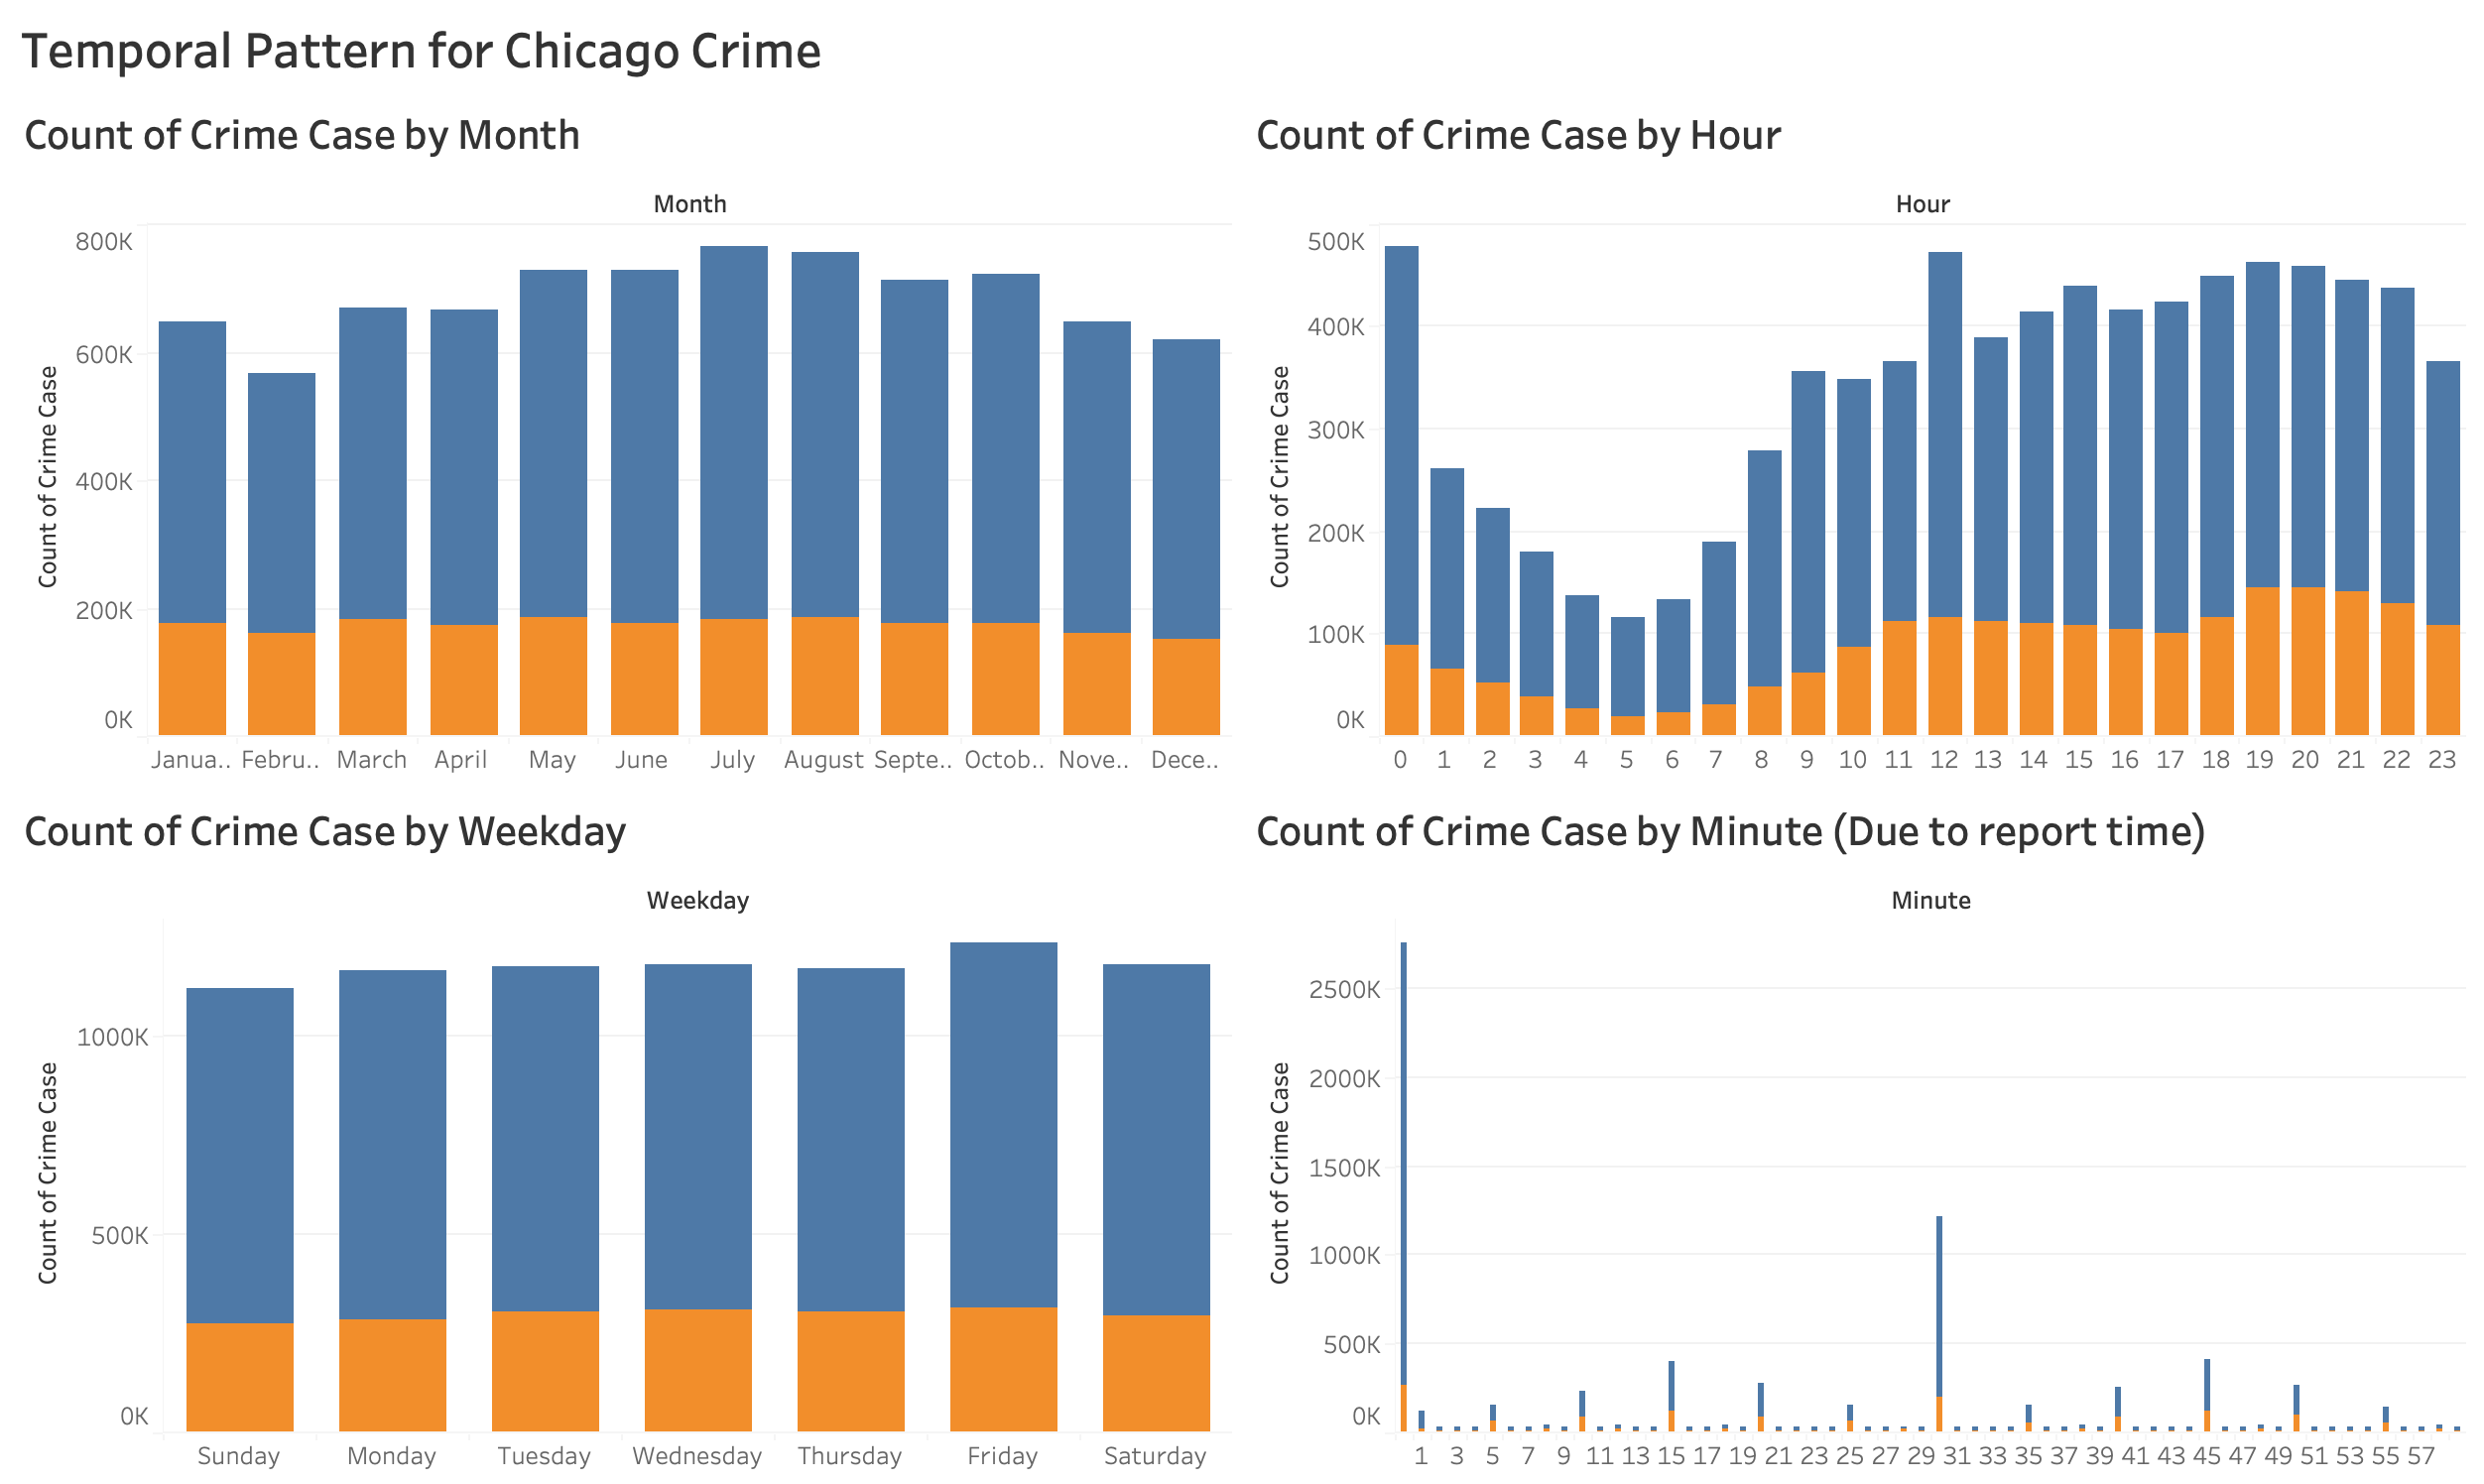
\includegraphics[width=\textwidth]{chart_time.png}
    \caption{Composite View of Temporal Crime Patterns.}
    \label{fig:chart_time}
\end{figure}

Analyzing Figure~\ref{fig:chart_time}:
\begin{itemize}
    \item The top-left chart displays monthly counts, revealing distinct seasonality. Crime incidents peak during warmer summer months (May-August) and decrease during colder months (lowest in February), suggesting an influence of weather or outdoor activity.
    \item The top-right chart illustrates hourly crime counts, demonstrating a clear diurnal cycle. Crime reports are minimal in the early morning (approximately 4-6 AM), increase throughout the day, with pronounced peaks at 12 PM (noon) and 24 PM (midnight).
    \item The bottom-left chart illustrates weekly counts. Crime levels appear relatively consistent across weekdays, potentially with a slight increase on Fridays.
    \item The arrest overlay, visible across these charts, suggests that arrests might constitute a slightly higher proportion during peak crime hours, although the overall number of reported cases vastly outweighs arrests for most periods.
    \item The bottom-right chart shows counts by minute, likely reflecting reporting artifacts (e.g., reports logged on the hour) rather than actionable crime patterns.
\end{itemize}

\subsection{Spatial Distribution of Crime}
\label{subsec:spatial_distribution}
Figure~\ref{fig:chart_space} illustrates where crimes are concentrated, examining both specific location types and broader geographical areas within Chicago.

\begin{figure}[htbp]
    \centering
    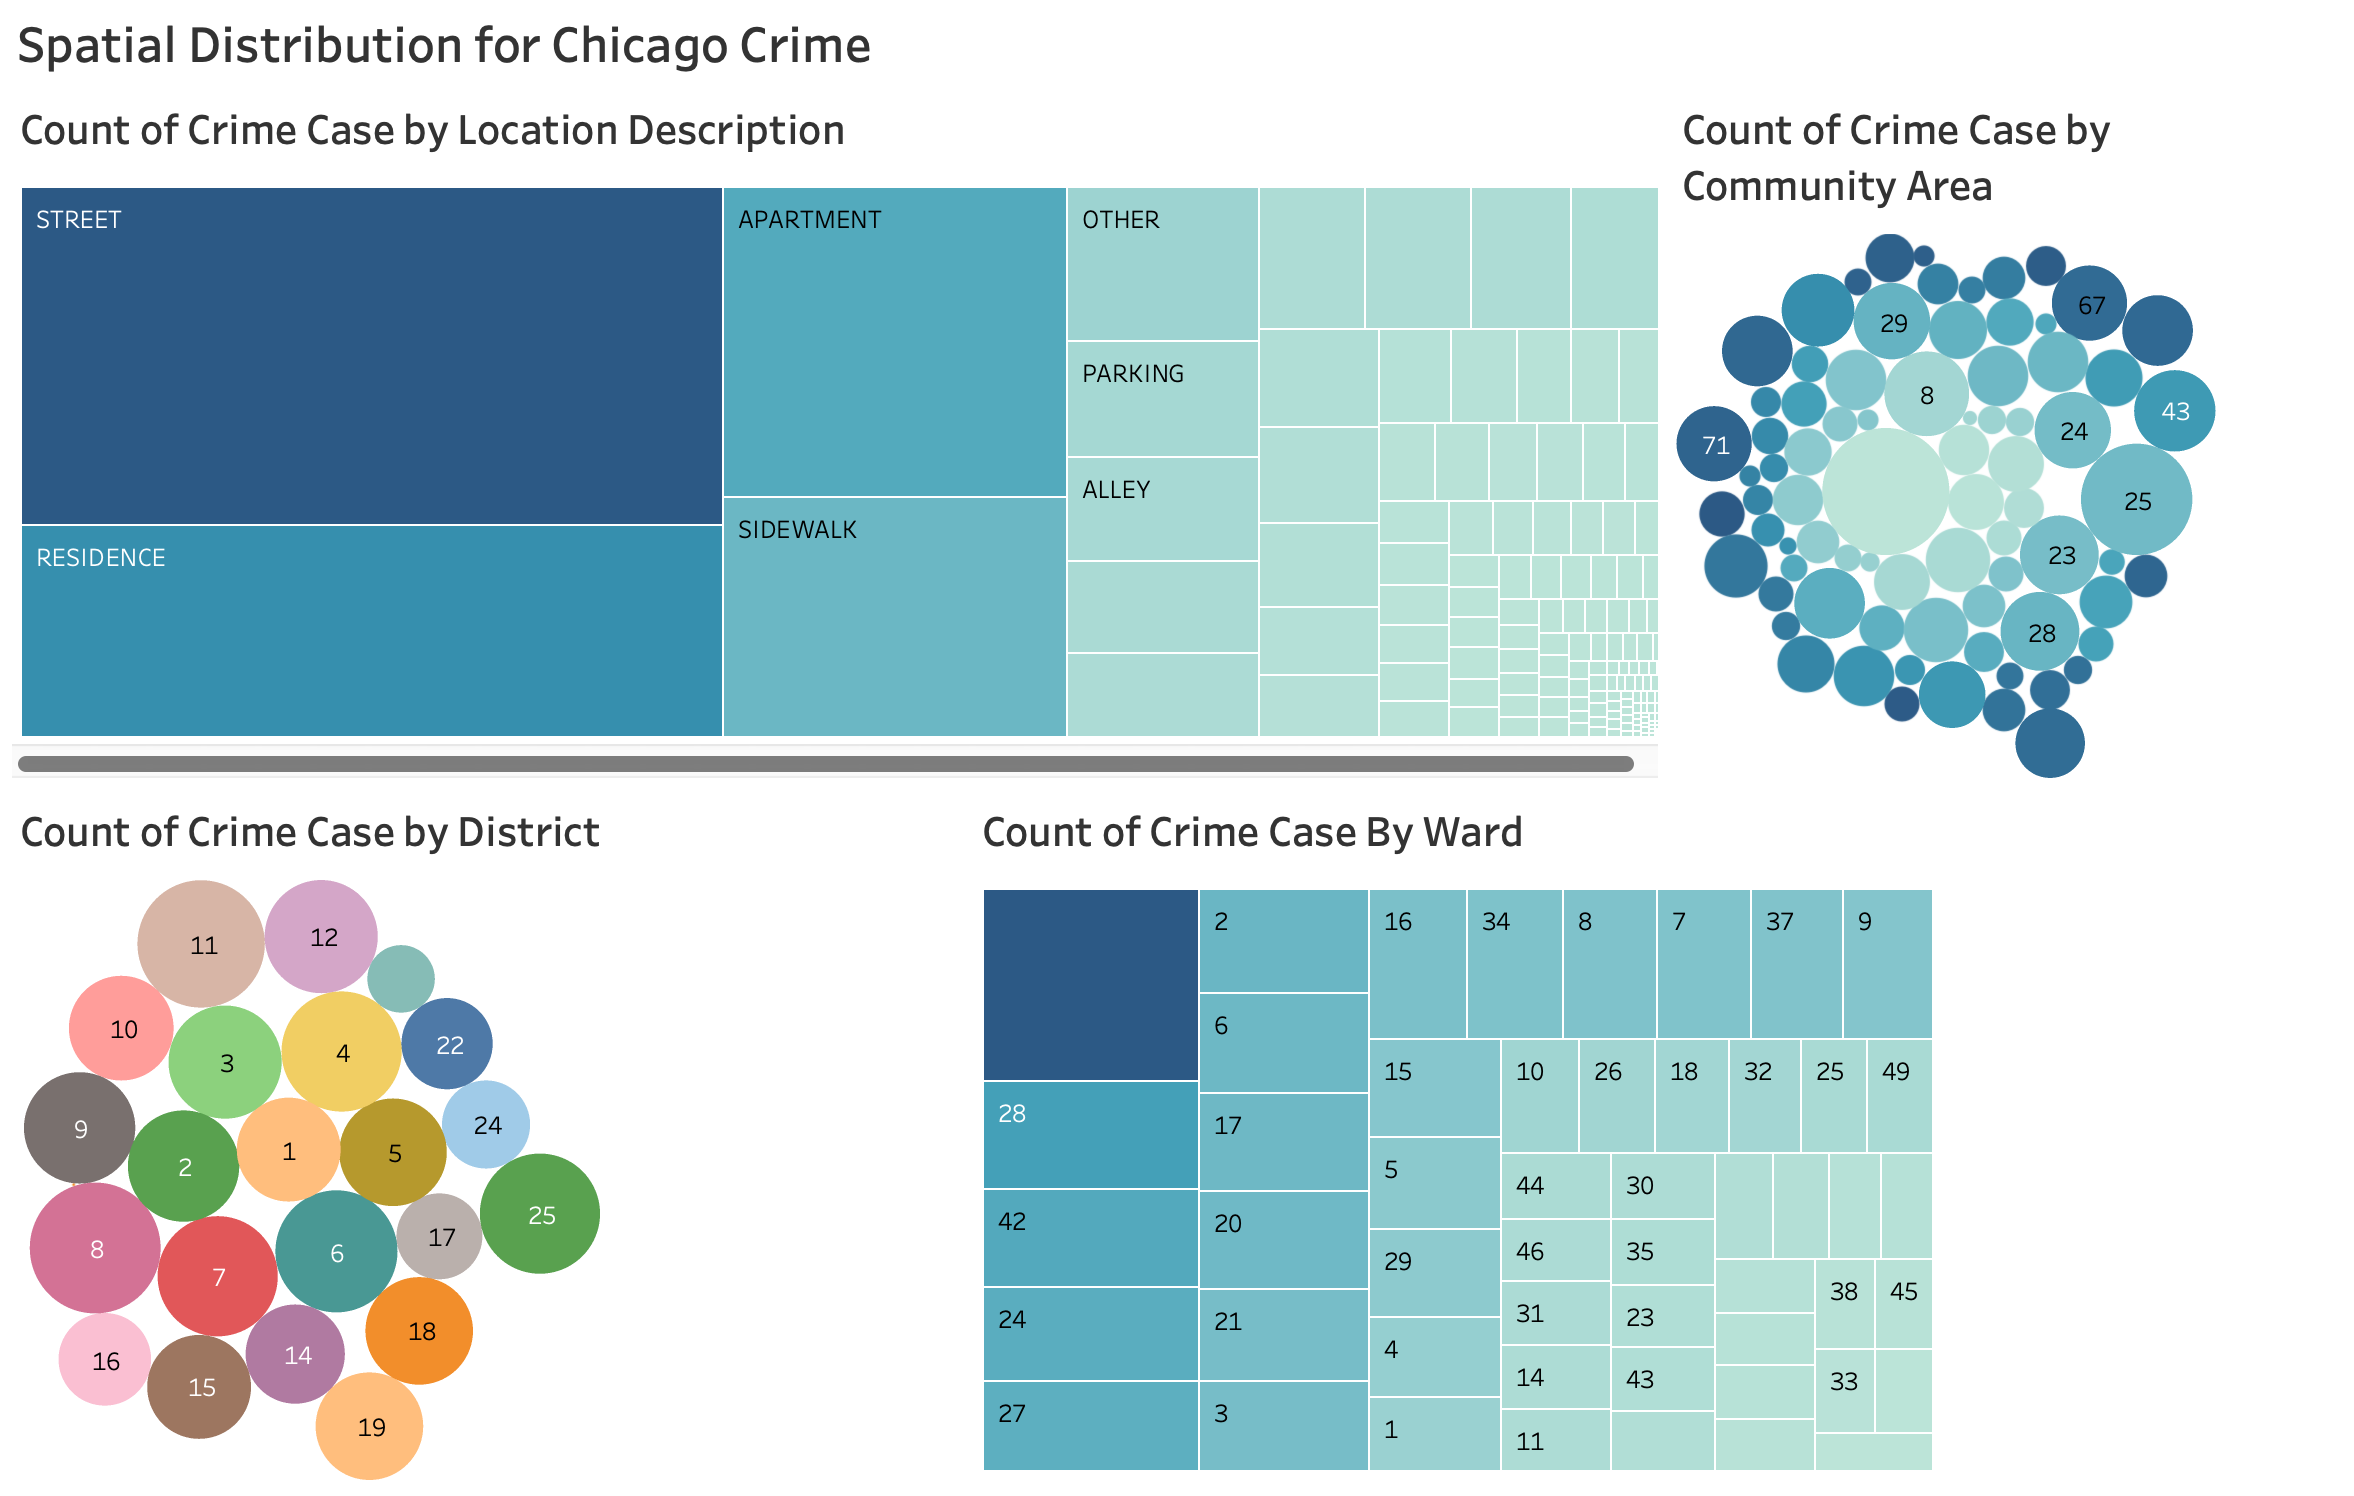
\includegraphics[width=\textwidth]{chart_space.png}
    \caption{Composite View of Spatial Crime Patterns.}
    \label{fig:chart_space}
\end{figure}

Analyzing Figure~\ref{fig:chart_space}:
\begin{itemize}
    \item A treemap (top-left) details common Location Descriptions. It shows crimes most frequently occur in public or accessible areas, predominantly on STREETs, followed by residential settings (RESIDENCE, APARTMENT) and SIDEWALKs.
    \item Geographical visualizations, including a bubble chart for Community Area (top-right), a bubble chart for District (bottom-left), and a treemap for Ward (bottom-right), demonstrate significant spatial concentration. Crime is not uniformly distributed; certain community areas, police districts, and wards bear a much higher burden of reported incidents than others, clearly indicating geographical hotspots."
\end{itemize}

\subsection{Correlation Analysis: Crime Type, Time, Location, and Arrests}
\label{subsec:correlation_analysis}
Beyond the general temporal and spatial trends, further analysis reveals correlations involving crime types. Visualizations breaking down crime counts by primary type over months and hours show that `THEFT` and `BATTERY` are dominant categories, largely driving the overall temporal patterns observed in Figure~\ref{fig:chart_time}. These detailed views can also reveal if specific crime types have unique peak times or seasonality.

Crime types are also strongly associated with specific locations. For instance, `THEFT` is particularly prevalent on `STREET`s and in retail environments, while `BURGLARY` is more common in `RESIDENCE`s, aligning with the locations identified in Figure~\ref{fig:chart_space}.

Finally, the relationship between crime type and arrest outcome is critical. Figure~\ref{fig:arrest_ratio} illustrates arrest ratios across different primary crime types. It highlights that while `THEFT` and `BATTERY` have the highest volumes, their arrest rates are relatively low compared to types like `NARCOTICS`, `HOMICIDE`, or `WEAPONS VIOLATION`. This disparity likely reflects differences in evidence availability, solvability, or policing priorities.

% Include ONE key correlation chart, e.g., Arrest Ratio.
\begin{figure}[htbp]
    \centering
    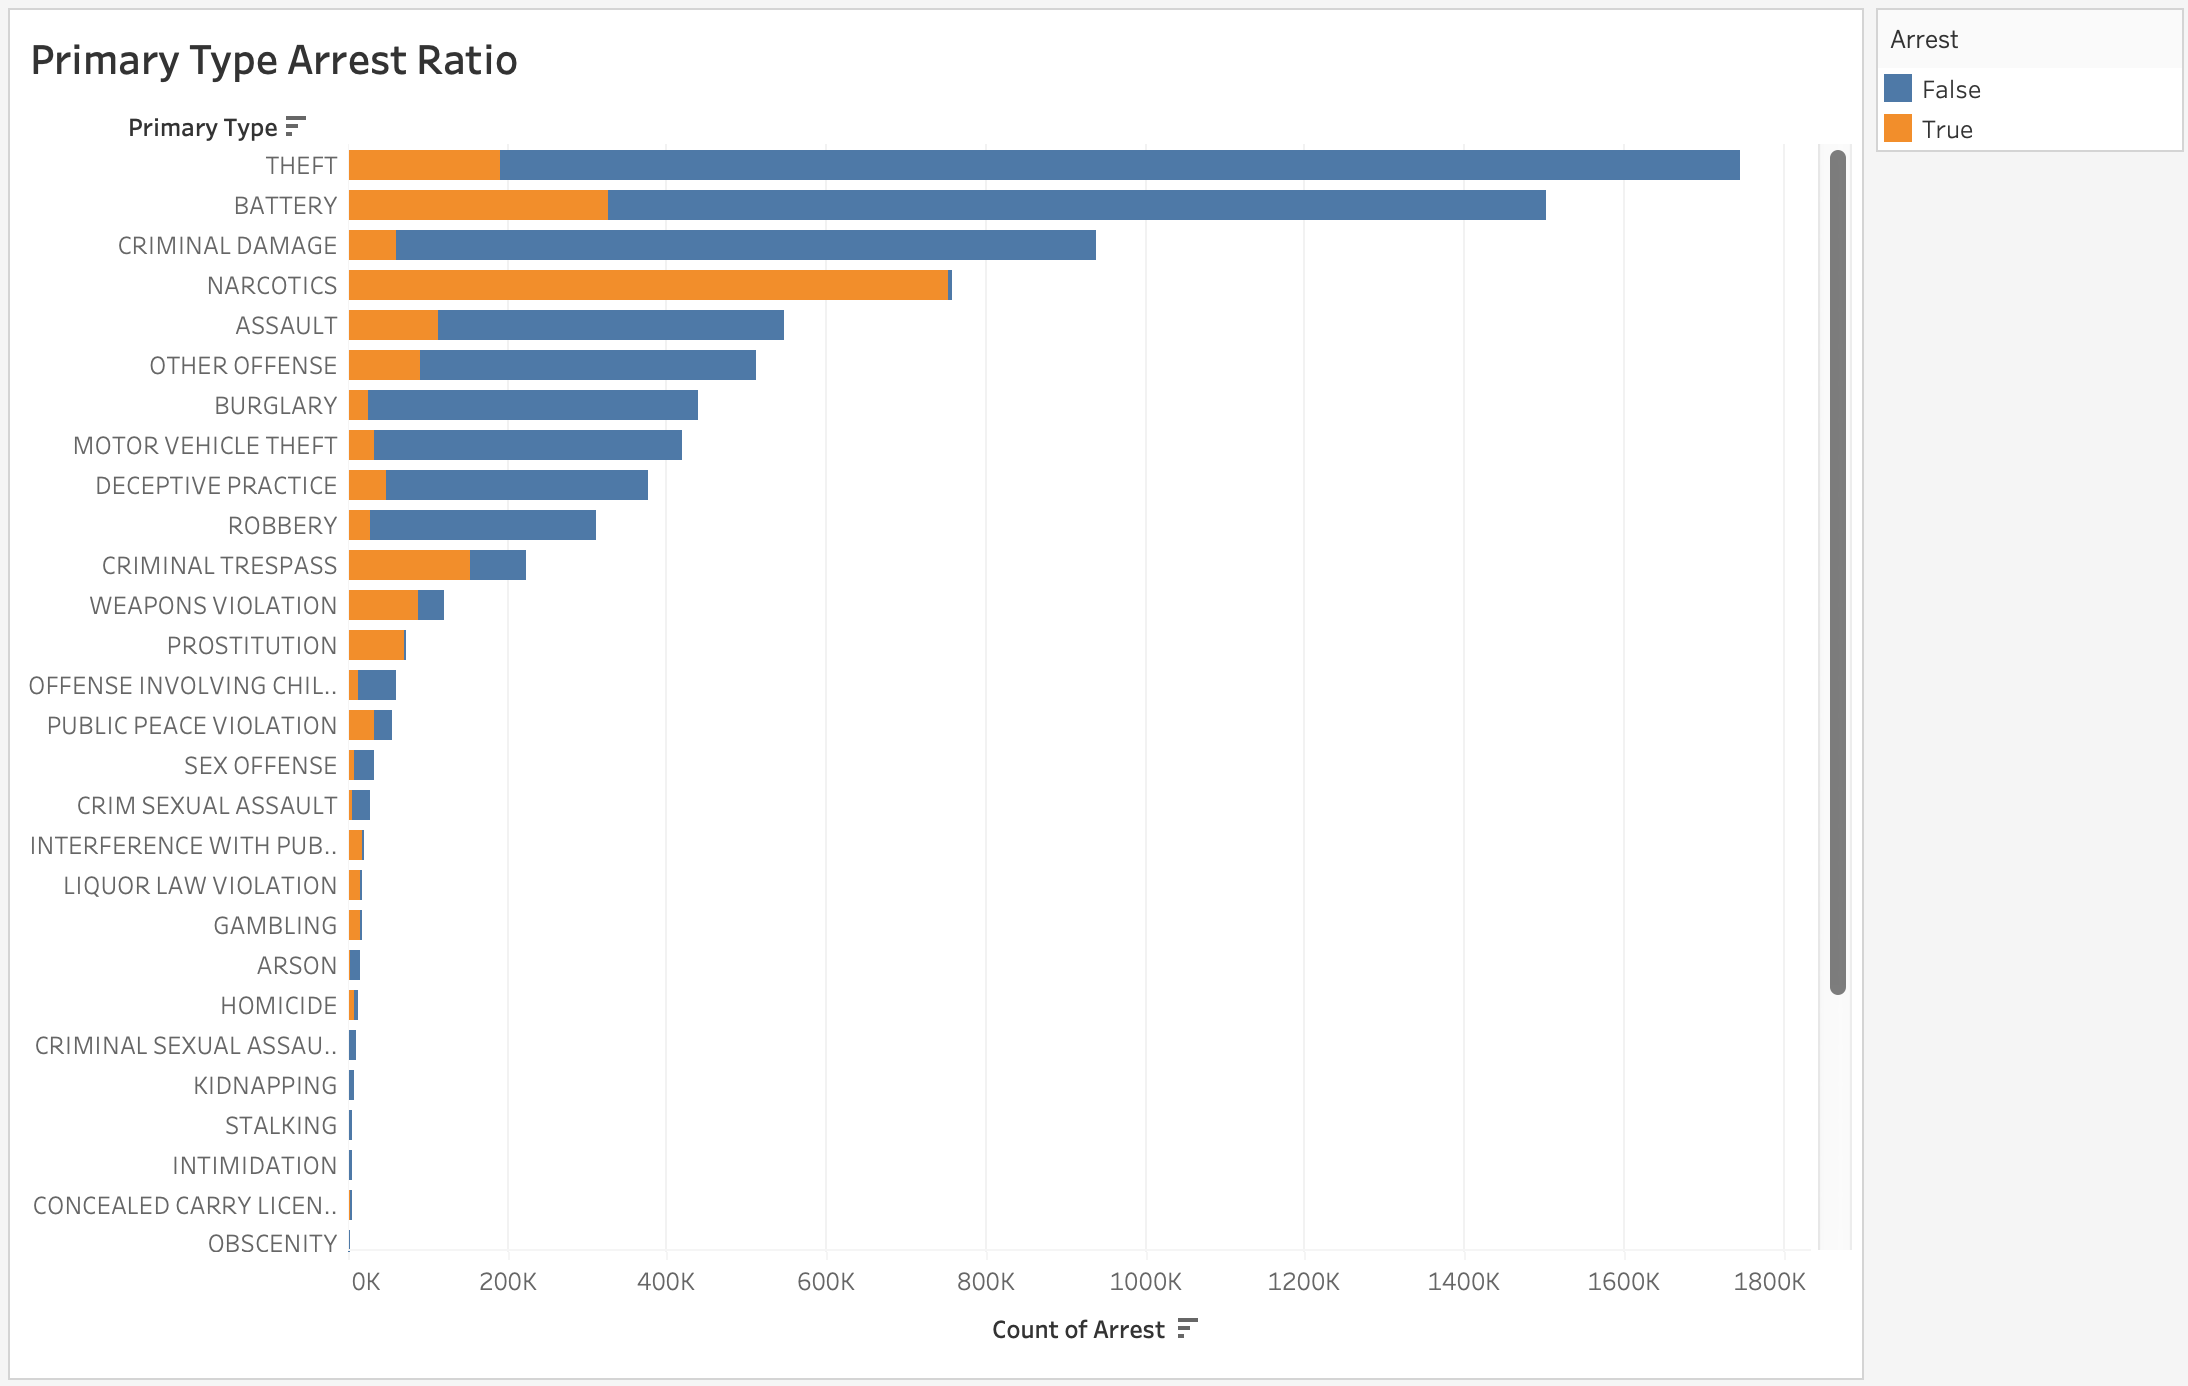
\includegraphics[width=0.9\textwidth]{chart_arrest_ratio.png} % Replace 'fig_arrest_ratio.png' with your filename for the Arrest Ratio chart
    \caption{Arrest Ratio by Primary Crime Type (Illustrative, based on Figure 6 in source PDF).}
    \label{fig:arrest_ratio}
\end{figure}

\subsection{Summary of EDA Findings}
\label{subsec:eda_summary}
The exploratory analysis highlights several core characteristics of the reported Chicago crime data:
\begin{itemize}
    \item Crime follows distinct temporal patterns, peaking seasonally in summer and diurnally in the afternoon/evening, with additional peaks observed at 12 PM (noon) and 24 PM (midnight) in the hourly distribution.
    \item Spatial distribution is highly uneven, concentrated in specific districts and common location types like streets and residences.
    \item `THEFT` and `BATTERY` are the most frequent crime types overall.
    \item Arrest rates vary significantly by crime type, not directly correlating with report volume.
\end{itemize}
These observations provide valuable context for understanding crime dynamics and guide further analysis and modeling efforts.


% \newpage

% \makeatother


\section{Preprocessing}
\label{sec:preprocessing}

\subsection{Introduction}
\label{subsec:preprocessing_intro}
This section presents the steps of data preprocessing of the Chicago crime dataset. The goal of data processing is to clean the dataset and prepare the data for future use in the model and prediction.

\subsection{Data Cleaning and Preparation}
\label{subsec:data_cleaning}
We performed a cleaning and preparation in the following steps:

S1: Read the dataset and use the data visualization methods to check the structure and attributes of the dataset.

S2: Identified missing values in critical columns such as Location Description, Latitude, and Longitude. 
For missing values in data cleaning, usually, we have three different ways to deal with this.

\begin{itemize}
    \item Drop missing value.
    \item Fill in the missing value with our own assumption.
    \item Train the model with existing value to predict missing value.
\end{itemize}

As shown in Figure~\ref{fig:missing_values}, the missing value ratio is low, and we chose to drop the missing value. Some features have very few missing values so that we cannot see them in the plot, so we use pandas to find exactly which are missing, then we drop these missing values in District, Location Description, X Coordinate, Y Coordinate, Latitude, Longitude, Location, Community Area, Ward. 

\begin{figure}[htbp]
    \centering
    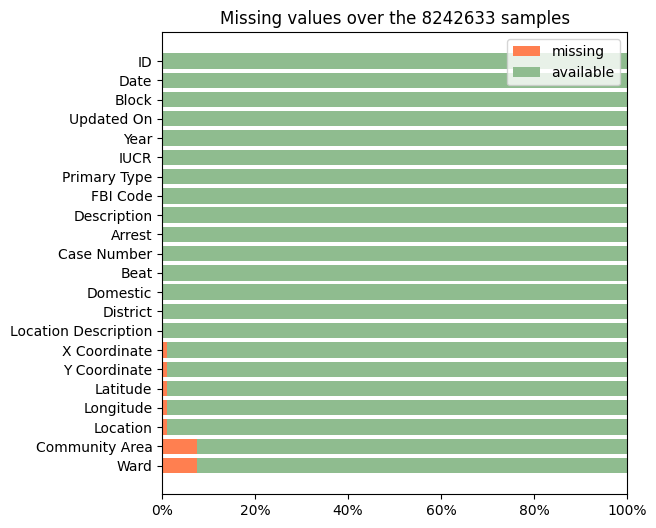
\includegraphics[width=0.8\textwidth]{missing_values.png}
    \caption{Missing values in the original dataset.}
    \label{fig:missing_values}
\end{figure}

S3: For data analysis in the future, we converted the date-time columns into a standardized format (DateTime) and transformed categorical variables into appropriate formats.

S4: Duplicate records were removed to maintain data integrity. Filtered out irrelevant or inconsistent data points.

Updated On, Year, Location, X Coordinate, and Y Coordinate were dropped as they either contained duplicate information or were not relevant to spatial analysis.

IUCR, FBI Code, and Description were removed since Primary Type already sufficiently represents crime categories.

Block and Location Description were removed as they provide overly specific location details, which are not useful for general crime prediction.

To enhance model generalizability, beat (the smallest police patrol area), District (comprising multiple beats), Ward (city council district), and Community Area (one of 77 Chicago community areas) were excluded. Instead, geographic coordinates were retained for spatial analysis using grid-based segmentation.

Domestic was removed as it is only relevant if predicting domestic crimes specifically.

The Primary Type was initially dropped because its utility in the modeling stage was uncertain. It can be reintroduced later if needed.

By removing these columns, the dataset becomes more structured, reducing noise and improving the efficiency of further analysis and predictive modeling.

\subsection{Remove Spatial Outliers}
\label{subsec:remove_spatial_outliers}
To better predict results, we conduct a shrinking tail to remove spatial outliers. Figure~\ref{fig:spatial_distribution}  illustrates the final results after this step. 

\begin{figure}[htbp]
    \centering
    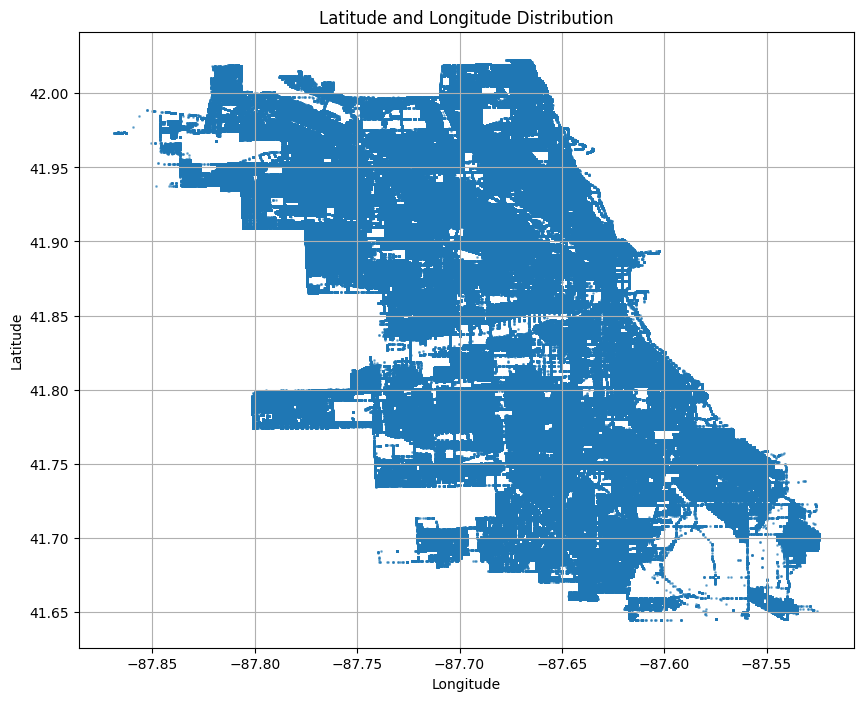
\includegraphics[width=0.8\textwidth]{spatial_distribution.png}
    \caption{Latitude and Longitude Distribution.}
    \label{fig:spatial_distribution}
\end{figure}

\subsection{Temporal and Spatial Aggregation}
\label{subsec:temporal_and_saptial_aggregation}
To simplify the dataset, and make it more structured and suitable for crime prediction models, we effectively incorporate spatial and temporal information.

\begin{itemize}
    \item Spatial Aggregation: Crime data is grouped into a 10×10 grid based on geographic coordinates, and the original latitude and longitude values are removed.
    \item Temporal Aggregation: The timestamp is standardized to hourly intervals to facilitate time-series analysis.
    \item Splitting Data by Arrest Status: Crime incidents are categorized into "arrest" and "not arrest" groups. A time-series dataset is constructed by counting crimes per grid and hour, ensuring that missing timestamps are filled with zero values.

\end{itemize}

\subsection{Summary of Data Preprocessing}
\label{subsec:preprocessing_summary}
These preprocessing steps significantly improved data quality, making it more suitable for analysis. The cleaned dataset can now be effectively used for crime pattern detection, trend analysis, and predictive modeling.

\end{document}